\section{Explaining Deep Models}

\begin{frame}[allowframebreaks]{Why Pixels and Tokens Are Harder}

    \begin{itemize}\small
        \setlength\itemsep{0.35em}
        \item There is no meaningful ``feature'' called pixel $(117,204)$. Attribution must be
              summarised over \textbf{regions}, or it is unreadable.
        \item There are hundreds of thousands of inputs, so coalition-based methods are far too
              expensive without a gradient shortcut.
        \item The inputs are strongly correlated by construction --- neighbouring pixels, adjacent
              tokens --- which is exactly the regime where independent perturbation misleads.
    \end{itemize}

    \vspace{0.5em}

    \begin{block}{Vanilla gradient saliency (Simonyan, Vedaldi \& Zisserman, 2014)}
        Take the score $s_c(x)$ for class $c$, backpropagate to the input, and display
        $\bigl|\partial s_c / \partial x\bigr|$ as an image.
    \end{block}

    \vspace{0.5em}

    \begin{itemize}\small
        \setlength\itemsep{0.3em}
        \item Interpretation: the pixels whose small changes would move the class score most.
              In practice raw gradients are \textbf{visually noisy} --- speckle rather than an object.
        \item Common repairs: \textbf{SmoothGrad} (average the gradient over noisy copies of the
              input) and \textbf{Integrated Gradients} (accumulate gradients along a path from a
              baseline to the input, restoring an additivity property analogous to SHAP's).
        \item Each needs a \textbf{baseline} or a noise level. As with SHAP's background, the
              choice changes the picture.
    \end{itemize}

    \vspace{0.3em}
    {\scriptsize K.~Simonyan, A.~Vedaldi and A.~Zisserman, ``Deep Inside Convolutional Networks:
    Visualising Image Classification Models and Saliency Maps,'' ICLR 2014 Workshop,
    \href{https://arxiv.org/abs/1312.6034v2}{arXiv:1312.6034v2}. M.~Sundararajan, A.~Taly and Q.~Yan,
    ``Axiomatic Attribution for Deep Networks,'' ICML 2017,
    \href{https://arxiv.org/abs/1703.01365v2}{arXiv:1703.01365v2}.}
\end{frame}

\begin{frame}{Grad-CAM: Class-Discriminative Heatmaps}

    \begin{columns}[T]
        \begin{column}{0.55\textwidth}
            \textbf{The idea, in three steps}
            \begin{enumerate}\small
                \setlength\itemsep{0.3em}
                \item Take the feature maps of the \textbf{last convolutional layer} --- they still
                      carry spatial position, but encode semantics.
                \item Weight each map by the average gradient of the target class score with
                      respect to that map (``how much does this channel matter for this class'').
                \item Sum the weighted maps, apply ReLU to keep positive evidence, and upsample to
                      the image size.
            \end{enumerate}

            \vspace{0.5em}
            \begin{itemize}\small
                \setlength\itemsep{0.25em}
                \item Coarse but \textbf{class-discriminative}: change the target class and the
                      heatmap moves.
                \item Works on any CNN without retraining; ViT variants exist.
                \item \textbf{Practitioner's use:} check that the heatmap sits on the object, and
                      not on a watermark, a ruler, a hospital tag, or the background.
            \end{itemize}
        \end{column}
        \begin{column}{0.43\textwidth}
            \centering
            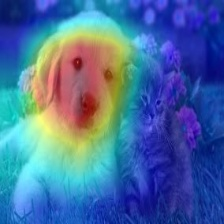
\includegraphics[width=0.47\linewidth,height=0.42\textheight,keepaspectratio]{images/responsible-ai/gradcam_resnet50_target_dog.jpg}%
            \hspace{0.02\linewidth}%
            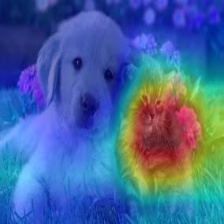
\includegraphics[width=0.47\linewidth,height=0.42\textheight,keepaspectratio]{images/responsible-ai/gradcam_resnet50_target_cat.jpg}

            \vspace{0.25em}
            {\scriptsize Same image, same network, two target classes: \emph{dog} (left),
            \emph{cat} (right).}

            \vspace{0.5em}
            {\scriptsize Source: example outputs from the
            \href{https://github.com/jacobgil/pytorch-grad-cam}{\texttt{pytorch-grad-cam}}
            library (ResNet-50). Method: R.~R.~Selvaraju, M.~Cogswell, A.~Das, R.~Vedantam,
            D.~Parikh and D.~Batra, ``Grad-CAM,'' ICCV 2017,
            \href{https://arxiv.org/abs/1610.02391v4}{arXiv:1610.02391v4}.}
        \end{column}
    \end{columns}
\end{frame}

\begin{frame}{Sanity Checks: A Pretty Heatmap Is Not Evidence}

    \begin{block}{Adebayo et al.\ (2018)}
        Two tests any saliency method should pass:
        \begin{itemize}
            \item \textbf{Model randomisation:} progressively randomise the trained weights. The
                  explanation should change.
            \item \textbf{Data randomisation:} retrain on randomly permuted labels. The explanation
                  should change.
        \end{itemize}
        They find that \textbf{some existing saliency methods are independent both of the model and
        of the data generating process} --- producing similar-looking maps regardless.
    \end{block}

    \vspace{0.8em}

    \begin{itemize}
        \setlength\itemsep{0.4em}
        \item Such a method is closer to an \textbf{edge detector} than to an explanation. It looks
              convincing because the object outline is where the edges are.
        \item Practical consequence: run the randomisation test yourself on the method you plan to
              ship. It costs one retraining run.
    \end{itemize}

    \vspace{0.3em}
    {\scriptsize J.~Adebayo, J.~Gilmer, M.~Muelly, I.~Goodfellow, M.~Hardt and B.~Kim, ``Sanity
    Checks for Saliency Maps,'' NeurIPS 2018,
    \href{https://arxiv.org/abs/1810.03292v3}{arXiv:1810.03292v3}.}
\end{frame}

\begin{frame}{``Attention Is Not Explanation'' --- and the Reply}

    \begin{columns}[T]
        \begin{column}{0.48\textwidth}
            \begin{tcolorbox}[colback=raiRed!5, colframe=raiRed!70,
                              title=Jain \& Wallace (NAACL 2019)]
                \scriptsize
                Across several NLP tasks:
                \begin{itemize}
                    \item Attention weights are frequently \textbf{uncorrelated} with
                          gradient-based importance.
                    \item One can construct \textbf{very different} attention distributions that
                          give \textbf{the same} prediction.
                \end{itemize}
                Conclusion: standard attention modules do not provide meaningful explanations and
                should not be treated as though they do.
            \end{tcolorbox}
        \end{column}
        \begin{column}{0.48\textwidth}
            \begin{tcolorbox}[colback=raiBlue!5, colframe=raiBlue!60,
                              title=Wiegreffe \& Pinter (EMNLP 2019)]
                \scriptsize
                The conclusion depends on what you mean by ``explanation.'' They propose four
                tests --- including a uniform-weight baseline and a diagnostic on frozen
                weights --- and find that adversarial attention distributions, where they exist,
                do poorly on the diagnostic.

                \vspace{0.4em}
                Attention is not \emph{no} evidence; it is not \emph{sufficient} evidence.
            \end{tcolorbox}
        \end{column}
    \end{columns}

    \vspace{0.9em}

    \begin{block}{What to do in practice}
        \centering
        \scriptsize Use attention maps as a \textbf{debugging view}, not as a justification shown to a
        user or a regulator. If you need an attribution for a transformer, use a method built for
        it (Integrated Gradients, attention rollout, gradient\,$\times$\,input) and validate it.
    \end{block}

    \vspace{0.2em}
    {\scriptsize S.~Jain and B.~C.~Wallace, ``Attention is not Explanation,'' NAACL 2019,
    \href{https://arxiv.org/abs/1902.10186v3}{arXiv:1902.10186v3}. S.~Wiegreffe and Y.~Pinter,
    ``Attention is not not Explanation,'' EMNLP 2019,
    \href{https://arxiv.org/abs/1908.04626v2}{arXiv:1908.04626v2}.}
\end{frame}
